
% REQUIREMENTS
% 2-8 pages!

% Deadline: Paper submission march 27th


% The paper must include references to relevant literature
% The paper must focus on a clearly described challenge goal
% Declare what part of the work is done solely for the purpose of this course.


% INCLUDING
% Motivation and goal
% Compare systems? (Difference between rdbms and graph database)
% Typical design and implementation - focus on graph database? Less on crawler and extraction of data.
% Performance evaluation?
% ...

\documentclass[conference]{IEEEtran}

% Package list
\usepackage{graphicx}
\usepackage[utf8]{inputenc}
\usepackage[backend=biber,
  bibstyle=ieee,
  citestyle=numeric-comp,
  sortcites=true]{biblatex}
\addbibresource{references.bib}

\begin{document}

% Title
\title{Title}

% Authors
\author{\IEEEauthorblockN{Andreas Isnes Nilsen}
\IEEEauthorblockA{
Department of Computer Science\\
UiT The Arctic University of Norway\\
Email: andreas.i.nilsen@uit.no}
\and
\IEEEauthorblockN{Nikolai Magnussen}
\IEEEauthorblockA{
Department of Computer Science\\
UiT The Arctic University of Norway\\
Email: nikolai.a.magnussen@uit.no}}
\maketitle

\begin{abstract}
There are a number of institutions in Norway conducting research, and an even larger number of units within those institutions.
In this paper, we introduce Cristin\cite{CRISTIN-about} where information is extracted by crawling researchers and their results, before inserting the information into a graph database.
This enable exploring the data and provide valuable insights into the research connectivity in Norway.
We discovered that top five institutions in Norway have great research connectivity between them.
Due to organizational structures, some institutions appear to be less connected across its units, displaying great connectivity within institutions as well for some, and inconclusive results for others.

\end{abstract}

% Introduction + motivation, goal, purpose
\section{Introduction}
Current research in Norway is abundant, but the amount of researchers co-authoring papers with researchers at different institutions or simply at different units at the same institution is not known.
To gain knowledge of this, we crawl Cristin, a public research information system for Norway, insert the data into a graph database, and execute carefully chosen queries to gain knowledge regarding research connectivity in Norway.


% Design
\section{Design}
This section describes shortly how the Cristin API was implemented. It then describes the process of crawling Cristins RDBMS. Finally, it describes how the extracted data was processed to create relations and nodes in a graph database.

% Skakke ha kake a kai
% Skrive en liten del om hvordan en henter ut data fra CRISTIN sitt API.
%	Rationale: Muliggjøre at en leser skal kunne reimplementere det vi har gjort
\subsection*{Cristin API}
Cristin provides APIs to extract information by querying a REST or Web Service API, which results in queries to the underlying RDBMS with more or less processing depending on the API buing used and endpoint queried\cite{CRISTIN-API-summary}.

The Web Service API\cite{CRISTIN-WS} is still available for legacy purposes, and enable querying for scientific results by a particular person. This functionality is not available in the more modern REST API. The REST API\cite{CRISTIN-REST} allow queries with less processing on the server's side than the Web Service API, but without the ability to query scientific results, such as papers in journals and presentations at conferences.

All data discussed later in the paper is extracted through these API's.

\subsection*{Crawling Cristin}
Authors are stored with ID's starting from 0, but with a large number of vacant person ID's, and the importance of relationship, makes rearching persons with monotonically increasing person ID infeasible.
Due to this limitation, a crawler is implemented. It will start at a person, retrieve the scientific results of that person, mark that person as crawled, store the results, and crawl each of the collaborating authors for all results retrieved that have not already been crawled, as to eliminate crawling cycles.
The number of authors to crawl will grow exponentially until all authors are finally crawled.

\subsection*{Processing extracted data}
Data extracted from Cristin is structured in json format which makes it easy to work with. Json objects are a key-value store which makes it similar to nodes in a graph database. Nodes are the entities in a graph database. They can hold any number of attributes (key-value-pairs) called properties. Nodes can be tagged with labels representing their different roles in your domain.\cite{neo4j} The difference between a json object and a node is that a json value can take form of a \textit{dictionary} and a property value can't. A json object is compatible as a node if none of the values are a dictionary and a label is attached to it.

\subsection*{Inserting data}
Inserting nodes into a graph database is straight forward, but creating relations between nodes can be a hassle. The challange is to know wether two nodes exists in the database before creating a relationship between them. \Fref{fig:subgraph} shows that the relationship \textit{guest} can't be created unless the green \textit{unit} node, red \textit{institution} node and the blue \textit{person} node exists in the database.

\begin{figure}[h]
  \centering
  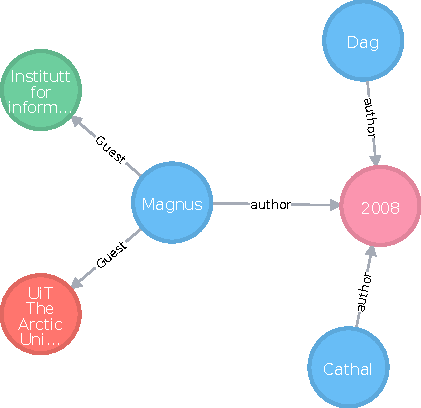
\includegraphics{graph.pdf}
  \caption{A subgraph}
  \label{fig:subgraph}
\end{figure}


% Kákékúngen
% Kanskje en idé å nevne terminologien vi bruker. (?)
% Hvor passer dette best?
\subsection*{Exploring data}
As previously mentioned, the goal of this paper is to show how people in the scientific community collaborate across units within the same institutions as well as across different institutions.
This can easily be modeled by using a graph database and the queries themselves as graph traversals.
We will argue both for the performance and for the ergonomy of the graph model provided by Neo4j over a RDBMS.


% Discussion
\section{Discussion}
As previously mentioned, we measure research connectivity as the collaboration between authors across units within the same organization and across different institutions.

\begin{figure}[h]
  \centering
  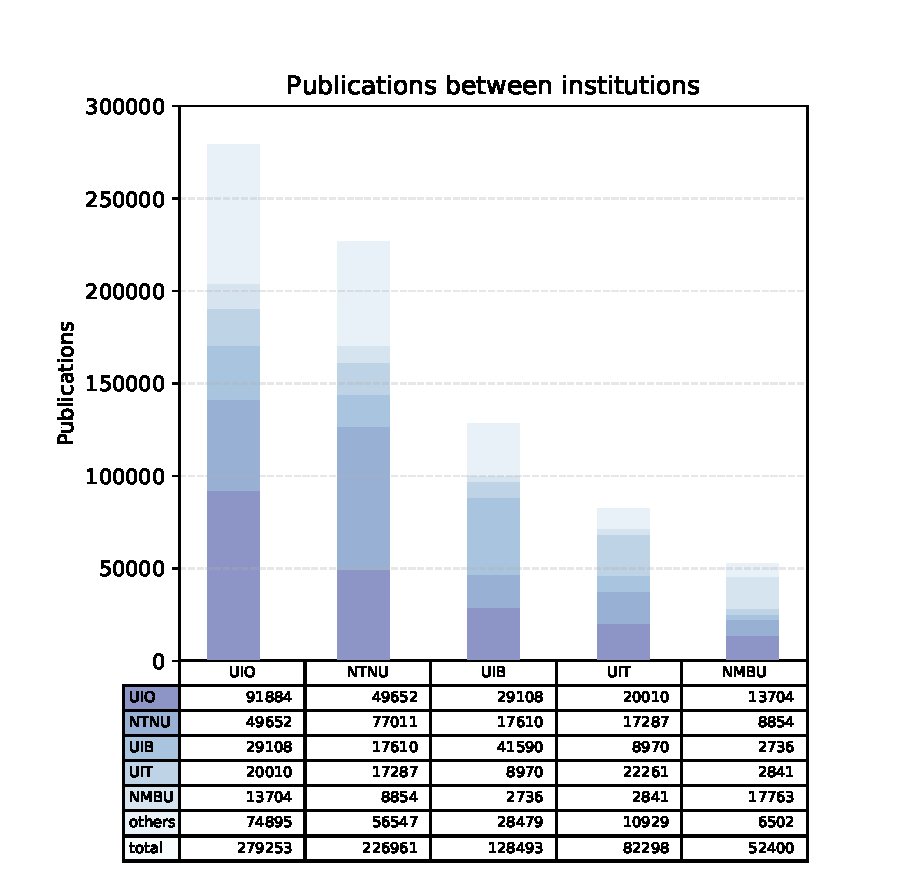
\includegraphics[width=0.48\textwidth]{table.pdf}
  \caption{Publications between institutions}
  \label{fig:result}
\end{figure}

\Fref{fig:result} shows UiO to be the institution with the greatest number of results, with NTNU following relatively close, and UiB, UiT and NMBU at much lower numbers.
An interesting observation is UiO’s cooperation with other institutions, among those, Oslo University Hospital, which they have a large number of joint results. Something that is not surprising.
Similarily, a large number of NTNU’s results are attributed to research in conjunction with UiO. This is expected as NTNU and UiO are the two largest institutions in Norway by far.


\begin{figure}[h]
	\centering
	\begin{tabular}{| l || c | c |}
		\hline
		Institution	& Only same institution	& Cross institution	\\ \hline
		UiO		& 0.329			& 0.671			\\
		NTNU		& 0.339			& 0.661			\\
		UIB		& 0.324			& 0.676			\\
		UiT		& 0.270			& 0.730			\\
		NMBU		& 0.339			& 0.661			\\
		\hline
	\end{tabular}
	\caption{Proportion of cross institution and only same institution results}
	\label{tab:institution-proportion}
\end{figure}

From \Fref{tab:institution-proportion}, we observe that all five institutions have more than $2/3$ of their results where the authors are employed at different institutions. UiT in particular is even higher than the other institutions, with close to 0.5 of it’s results being in coordination with either UiO or NTNU. As with UiT, NMBU has a large part of it’s results in conjunction with UiO, probably due to them being located relatively close to one another. Why then, UiT is so heavily influenced by the research at UiO and NTNU, is not known.

\begin{figure}[h]
	\centering
	\begin{tabular}{| l || c | c |}
		\hline
		Institution	& Only same unit	& Cross unit	\\ \hline
		UiO		& 0.226			& 0.774		\\
		NTNU		& 0.543			& 0.457		\\
		UIB		& 0.505			& 0.495		\\
		UiT		& 0.320			& 0.680		\\
		NMBU		& 0.661			& 0.339		\\
		\hline
	\end{tabular}
	\caption{Proportion of cross unit and only same unit results}
	\label{tab:unit-proportion}
\end{figure}

In \Fref{tab:unit-proportion}, we see that UiO is the institution who has the highest proportion of published results across units, surprisingly NTNU has the lowest proportion together with NMBU. An important observation is that UiO has 669 registered units against NTNUs 97 registered units and NMBUs 16 registered units, and as mentioned above NTNU and UiO are largest institutions in Norway. The reason for NTNUs and NMBUs low proportion of published results across units is that they have a higher rate of persons per units then institutions like UiT and UiO with a low rate of persons per units.


% Implementation
\section{Implementation}
The crawler and system for inserting data into the graph database is implemented using python.
Neo4j 3.3 is the graph database used for storing and querying the data.


% Evaluation
\section{Evaluation}
There are a number of ways to evaluate research connectivity, but for this paper, the following data is examined.
The total number of publications authored at the five top publishing institutions in Norway, and whether or not they are subject to cooperation between researchers from different institutions, such as UiO and NTNU.
This will be a measure of the connectivity between institutions in Norway, and it remains to measure the connectivity within institutions.
Connectivity within institutions can be measured in much the same way, but rather than determining if results have been subject to cooperation between researchers from different institutions, we want to determine if they are produced by persons within the same institutions but from different units of that institution, such as a different faculty, or a different department.


% Conclusion
\section{Conclusion}
Through Cristin, there are large amounts of data available, which is extracted and inserted into a graph database to perform the queries for the purpose of examining research connectivity in Norway.
As the experimental results show, the research connectivity between institutions is great, around 2/3 of the results are collaborartions between authors from different institutions.
Relating this to connectivity within institutions and thus, between units of those institutions, the connectivity is very different from institution to institution.
This is most likely due to the different organizational structures of the institutions, where some institutions, such as UiO and UiT, comprise a large number of units while others, such as NTNU and NMBU are made up of far fewer units, leading to the inconclusive results.


\printbibliography

\end{document}
